\subsubsection{Minuta de reunião (07-Janeiro-2016)}

\begin{tabbing}
  Local \= xxx \kill
  Local \> : LEAD \\
  Data  \> : 07 de Janeiro de 2016 \\
  Hora  \> : 10:00
\end{tabbing} 

%---------------------------------------------------------------------
\participantes{
  \gabriel,
  \julia,
  \estevão,
  \elael,
  \renan,
  \ramon.

}

\textbf{Aprovação da minuta}

\textbf{Update semanal do Projeto EMMA}

\begin{itemize}
			\item Definir datas e entregáveis para o final do EMMA com ESBR.
			\item Feedback RIJEZA para SHUTTER.
			\end{itemize}
   									
						
\textbf{\gabriel.} 
	\begin{itemize}
			\item Pesquisa ‘Oclusão’: encontrou simulador de laser scan para criar cenas
			de oclusão e testas algorítmos.
			\end{itemize}
		
		\item \textbf{Novas tarefas:}
			\begin{itemize} 
				\item Trabalho em andamento do com Point Cloud e PCL.
			\end{itemize}

					
   \textbf{\estevão.} 
	\begin{itemize}
		\item \textbf{Tarefas concluídas:}
			\begin{itemize}    
			    \item Adicionar grau de liberdade em Y na base.
			    \item Cotaçõa Motoman encaminhada.
				
			\end{itemize}
		
		\item \textbf{Novas tarefas:}
			\begin{itemize} 
			    \item Desenhar ambiente com 5 pás da Usina Santo Antônio.
			    \item Retomar com Rijeza o projeto do Shutter, vai preparar um diagrama
			    explicativo com o conceito da solução.
			\end{itemize}
	\end{itemize}

	
	  \textbf{\elael.} 
	\begin{itemize}
		\item \textbf{Tarefas concluídas:}
			\begin{itemize}    
				\item Artigo EMMA-DETAIL 2: organizou conteúdo e estrutura, re-leu os
				artigos anteriores e terminou introdução.
			\end{itemize}
		
		\item \textbf{Novas tarefas:}
			\begin{itemize} 
			    \item Dar continuidade ao artigo do EMMA-DETAIL.
			\end{itemize}
	\end{itemize}			
			
  \textbf{\renan.} 
	\begin{itemize}
		\item \textbf{Tarefas concluídas:}
			\begin{itemize}    
				\item Relatório de simulaçòes do Open Rave e MoveIt
			\end{itemize}
		
		\item \textbf{Novas tarefas:}
			\begin{itemize} 
			    \item Ver revisão de artigo com Ramon.
			\end{itemize}
	\end{itemize}	
			
   \textbf{\julia.} 
	\begin{itemize}
		\item \textbf{Tarefas concluídas:}
			\begin{itemize}    
				\item Conteúdo para artigo para EMMA-UI. 
				\item cobrar testes do grupo formado para questionários da pesquisa.
			\end{itemize}
		
		\item \textbf{Novas tarefas:}
			\begin{itemize} 
			    \item Resultados de questionários.
			    \item formato de artigo conferido por Ramon.
			\end{itemize}
	\end{itemize}		



\textbf{Agenda para a próxima reunião:}
  \begin{itemize}
    \item Resultado de pesquisas individuais.
    \item Novas tarefas \& recomendações.
  \end{itemize}


\vspace{5mm}%
\parbox[t]{70mm}{
  Aprovado por: \\[5mm]
  \centering
  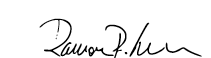
\includegraphics[width=65mm]{figs/logo/assinatura-ramon.png} \\[-4mm]
  \rule[2mm]{70mm}{0.1mm} \\
  \ramon \\[1mm]
  Coordenador do Projeto \\
}

%---------------------------------------------------------------------
\fim